\documentclass[final,5p,times,twocolumn]{elsarticle}

\usepackage{amsmath,amssymb,booktabs,multirow,graphicx,xcolor,url}
\usepackage[caption=false,font=small]{subfig}
\usepackage{threeparttable}
\usepackage{enumitem}
\usepackage{microtype}
\usepackage{float}
\usepackage{hyperref}
\hypersetup{colorlinks=true,linkcolor=blue!55!black,citecolor=blue!55!black,urlcolor=blue!55!black}
\graphicspath{{figures/}}
\journal{Applied Ocean Research}

\begin{document}
\raggedbottom
\begin{frontmatter}

\title{Supervision-Associated Expert Complementarity and Temporal Model-Hierarchy Changes in Coastal Sea-Level Residual Forecasting}

\author[anon]{Anonymous Author(s)}
\address[anon]{Affiliation withheld for double-anonymous review}

\begin{abstract}
Non-tidal coastal sea-level residuals are harder to forecast than tide-dominated total water levels and expose whether a model has learned meteorological and oceanographic departures. We study direct 24-h residual forecasting using hourly water-level, atmospheric, current, wave, local-meteorological, and bathymetric variables. Development uses seven northeastern United States stations; a prospectively locked spatial confirmation uses ten non-overlapping Delaware Bay--River stations. Graph WaveNet is the strongest deep backbone. Eta-only and multistate experts alternate in lead-wise dominance in the original-region refit (13 versus 11 leads), but this pattern does not transfer: multistate wins 22 of 24 leads and all ten stations externally. A fixed low-degree-of-freedom dual expert, HS-DT-GWN, retains positive external sequence effects over eta-only ($+0.0163$) and multistate ($+0.0045$); the latter 168-h block interval crosses zero. VARX-Ridge remains the strongest external sequence model (0.7657 versus 0.6803 for mean HS-DT run skill), yet the five-seed mean curves change order by lead: HS-DT trails VARX over Leads 1--8 but exceeds it at Lead 24. Two of three locked replication criteria pass. Matched physical-prior effects remain small and mixed. The evidence therefore supports low-complexity deep-expert complementarity and horizon-dependent model-family ranking across regions, while showing that supervision structure is region-dependent and that physical-prior utility is conditional rather than universal.
\end{abstract}

\begin{keyword}
coastal sea level \sep non-tidal residual \sep Graph WaveNet \sep expert complementarity \sep temporal robustness \sep physics-informed machine learning
\end{keyword}
\end{frontmatter}

\section{Introduction}
Astronomical tide is predictable enough to be issued operationally, but observed coastal water level also contains departures driven by wind, pressure, shelf circulation, currents, waves, local geometry, and observation error. Let observed total water level be $z_{i,t}$ and predicted astronomical tide be $T_{i,t}$. We forecast the non-tidal residual
\begin{equation}
\eta_{i,t}=z_{i,t}-T_{i,t},
\label{eq:residual}
\end{equation}
for every station $i$ and each of the next 24 h. Total water level can subsequently be reconstructed as $\hat z_{i,t+h}=T_{i,t+h}+\hat\eta_{i,t+h}$. This prevents the predictable tide from dominating the reported skill.

Deep temporal models can learn nonlinear forcing--response relationships, while graph neural networks share information along spatially related stations \citep{kipf2017gcn,li2018dcrnn,wu2019graphwavenet}. Physics-informed learning can add process-inspired features, soft residuals, or hybrid corrections \citep{raissi2019pinn,karniadakis2021piml}. However, a larger hybrid score does not establish which component helped. Architecture, auxiliary supervision, additional trainable capacity, test-aware selection, and forcing availability can all confound attribution.

Our experiments initially followed the common progression from a graph recurrent model to physical residual regularization. Stronger baselines and later temporal evaluations changed the scientific question. The paper now asks:
\begin{enumerate}[leftmargin=*,itemsep=1pt]
\item How much skill comes from the spatiotemporal backbone rather than an added physical penalty?
\item Is multistate supervision associated with horizon- or station-specific expert behavior?
\item Can a frozen low-complexity expert combination transfer across time periods?
\item Why does a strong linear model dominate some periods and fail at far leads in others?
\item Does physical information retain measurable value under same-capacity controls?
\end{enumerate}

The principal contribution is therefore a controlled evidence framework, not a claim that one complex model wins every metric. We provide (i) a strong GNN-to-Graph-WaveNet architecture ladder; (ii) a horizon specialization index, expert-error correlation, and station-by-horizon analysis; (iii) a fixed HS-DT expert combination evaluated across multiple periods and a non-overlapping ten-station region; (iv) a matched VARX--deep comparison revealing period- and horizon-dependent hierarchy changes; and (v) a backbone-by-injection physics utility matrix that includes negative controls and failed high-capacity extensions. The spatial confirmation separates transferable complementarity from non-transferable station-wise specialization.

\begin{figure}[t]
\centering
\subfloat[Residual forecasting task.]{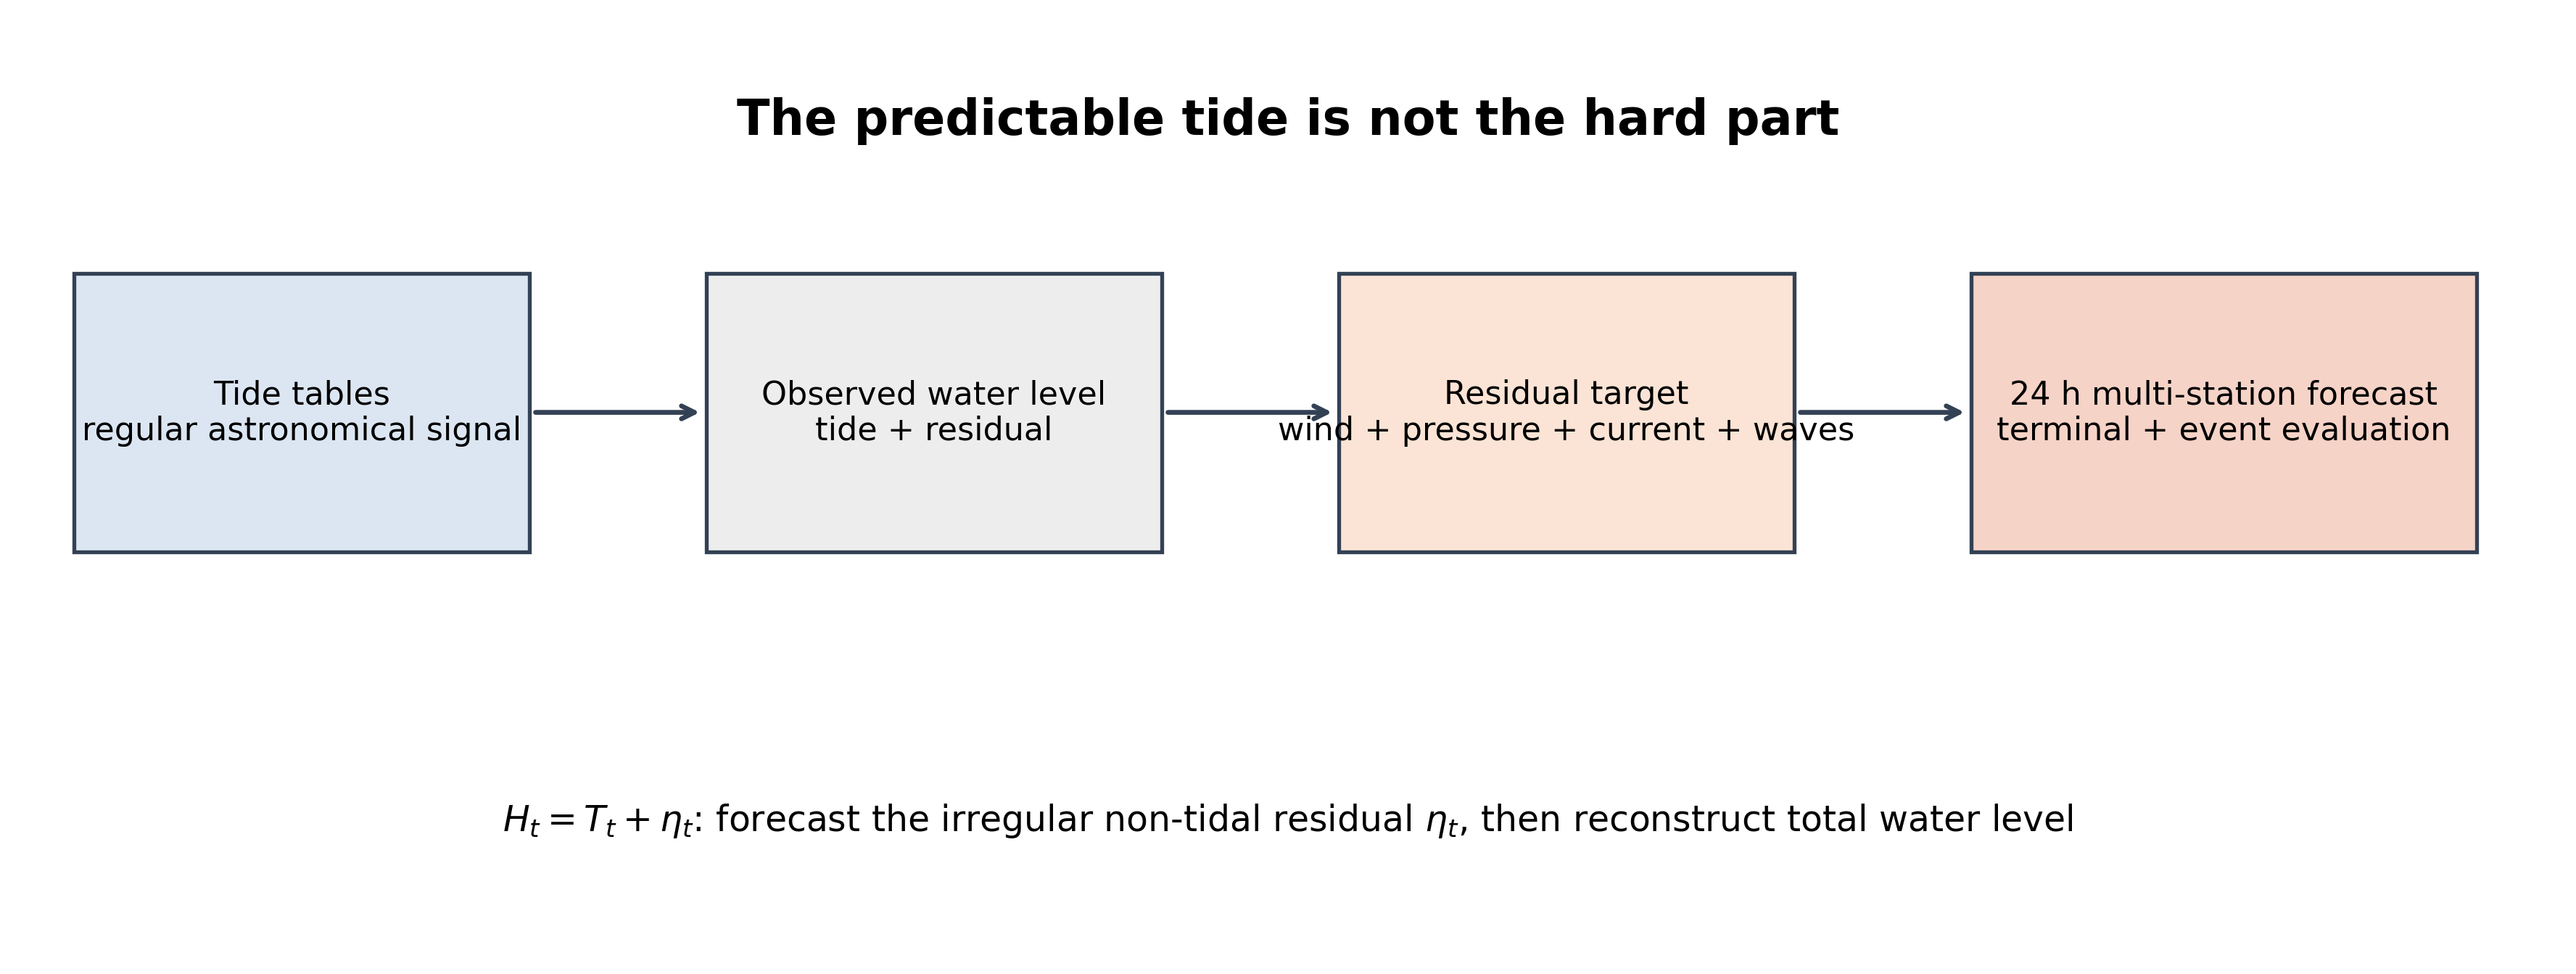
\includegraphics[width=0.48\linewidth]{fig1_problem_story.png}}\hfill
\subfloat[Seven-station coastal graph.]{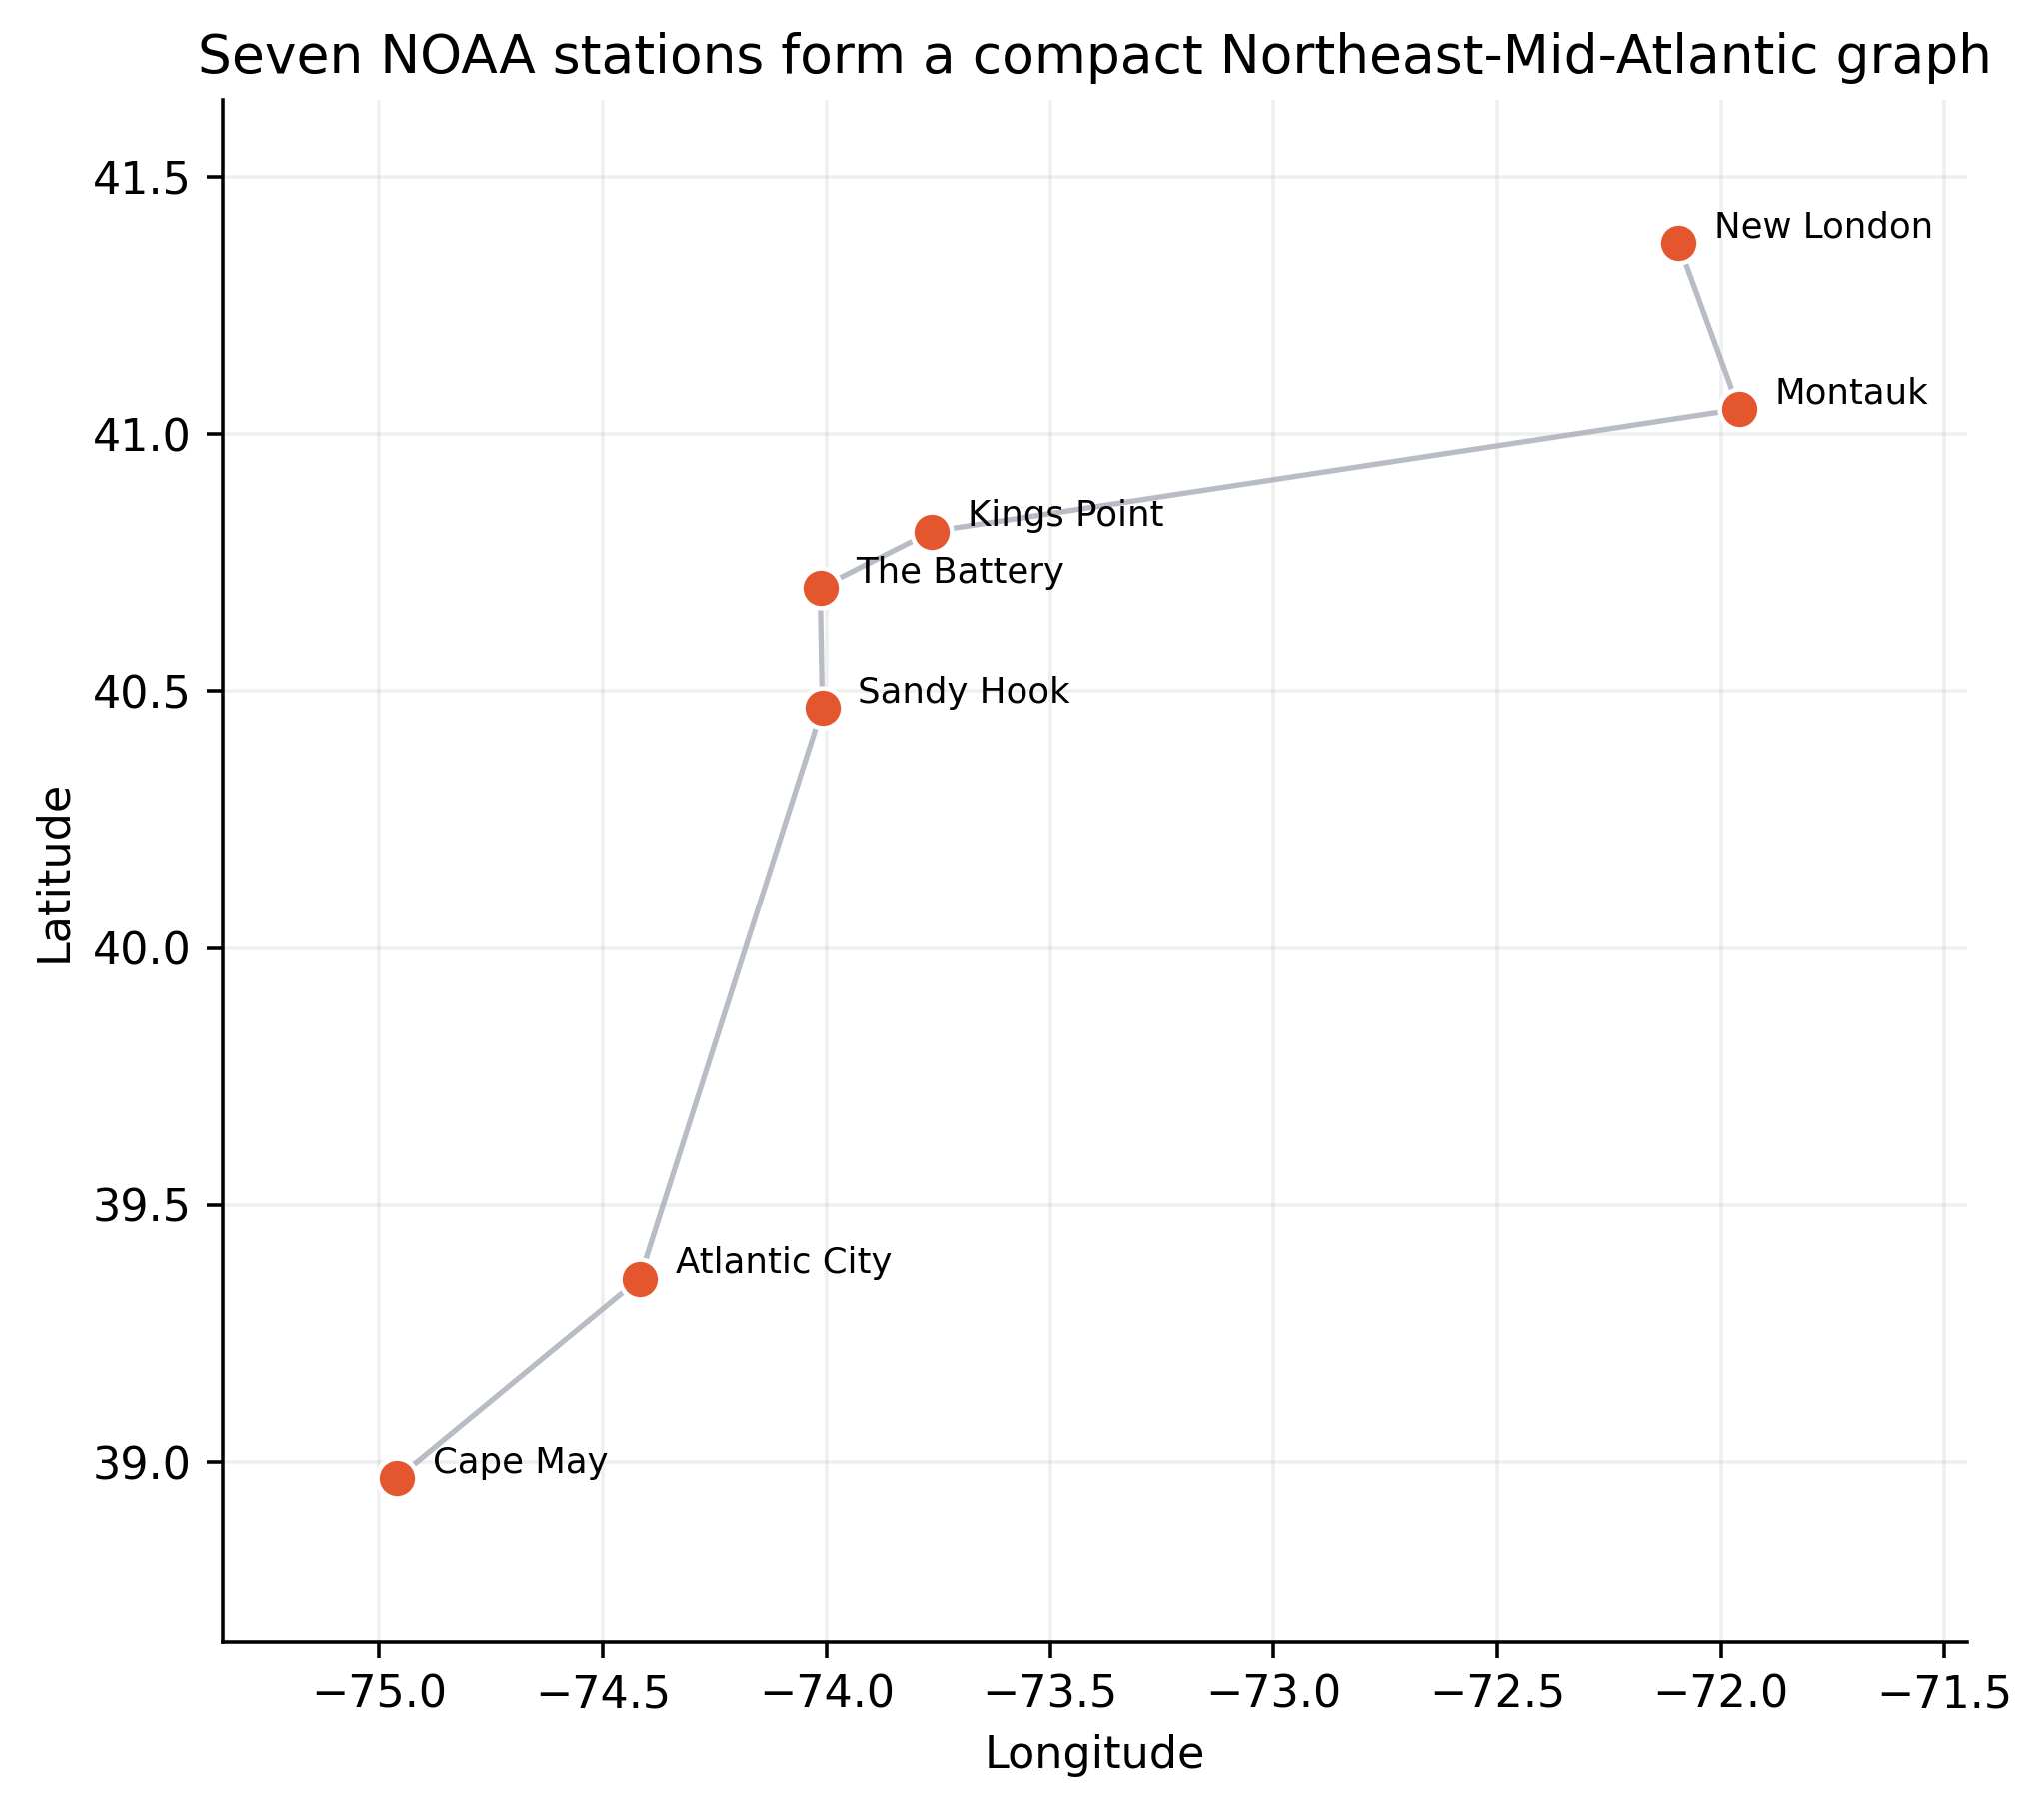
\includegraphics[width=0.48\linewidth]{fig2_station_network.png}}
\caption{Study setting. The target is the non-tidal residual rather than tide-dominated total water level. Stations span the New Jersey, New York, and Connecticut coast.}
\label{fig:setting}
\end{figure}

\section{Related work}
Operational tide prediction and hydrodynamic surge models exploit different sources of predictability. Hydrodynamic systems retain explicit governing dynamics but require atmospheric and boundary forcing, bathymetric resolution, and calibration; comprehensive coastal sea-level observing and modelling systems therefore combine multiple measurement and process-model components \citep{ponte2019coastal}. Machine learning has been used for direct surge prediction, spatial-field emulation, model-error correction, and ensemble forecasting \citep{salighehdar2017ensemble,xie2023surge,bai2022surge,giaremis2024lstm,qin2023review}. Related work also uses neural networks for regional sea-level change and global coastal-extreme estimation, tasks that are scientifically adjacent but distinct from short-horizon residual forecasting \citep{nieves2021regional,bruneau2020extremes}. Graph formulations are attractive for connected coastal observations because they combine node-wise temporal histories with learned or prescribed spatial dependence \citep{jiang2024causal,li2018dcrnn,wu2019graphwavenet}. In the wider spatiotemporal literature, temporal graph convolutions and learned graph structure have improved multivariate forecasting when dependencies are not known a priori \citep{yu2018stgcn,wu2020mtgnn,jin2024gnntimeseries}. Coastal gauges differ from traffic sensors, however: the graph is small, forcings are heterogeneous, and tide removal makes the remaining target more nonstationary.

Direct multi-horizon forecasting avoids recursive error accumulation but makes horizon-specific behavior and auxiliary-task interference important \citep{lim2021tft}. Multitask learning can improve shared representations, but task relatedness and loss weighting determine whether auxiliary supervision helps or interferes \citep{caruana1997multitask,kendall2018multitask}. We therefore describe the expert differences as supervision-associated and test them by station and lead rather than assuming a universal multitask benefit. Forecast combination has long shown that imperfect predictors can improve when their errors are not identical \citep{bates1969combination,clemen1989combining}; learned mixtures generalize this idea but add estimation freedom \citep{jacobs1991moe,monteromanso2020fforma}. HS-DT is intentionally closer to a fixed forecast combination than to a trainable router: this limits selection freedom while testing whether two supervision regimes leave exploitable error differences.

Out-of-time assessment is essential because random or single historical splits can misstate future forecasting performance \citep{cerqueira2020evaluation,hewamalage2023pitfalls}. Strong linear models can rival much larger architectures in long-horizon benchmarks \citep{zeng2023dlinear}, reinforcing the need to evaluate model families rather than presume a deep-learning advantage. Forecast comparisons should distinguish scale-sensitive errors, relative skill, and target variance \citep{hyndman2006accuracy}, and large forecasting competitions likewise show that no single complexity class dominates every series \citep{makridakis2018m4}. We therefore separate retrospective reconstruction, chronological refit, frozen evaluation, and diagnostic overlay rather than pooling them as equivalent evidence. This tiering is especially important for the VARX--deep comparison because the 2026 VARX overlay was designed after those target outcomes had been viewed.

Physics-informed and theory-guided machine learning range from equation residuals to hybrid features and learned closures \citep{karpatne2017theory,reichstein2019earth,karniadakis2021piml,willard2022scientific}. A recent storm-surge case study illustrates the appeal of physics-informed neural modelling when the governing-domain information is available \citep{zhu2025pinnsurge}. Sparse tide gauges, by contrast, do not identify a full shallow-water partial differential equation: spatial derivatives, boundary conditions, and bathymetry are incompletely observed. We consequently treat graph-discretized dynamic residuals and ODE-inspired channels as simplified priors. Their value must be measured against matched no-physics and same-capacity controls.

\section{Data and evidence protocols}
\subsection{Stations, inputs, and target}
The network contains New London, Montauk, Kings Point, The Battery, Sandy Hook, Atlantic City, and Cape May. The 2023--2025 hourly data combine NOAA CO-OPS water level and tide \citep{noaa_tides}, ERA5 wind and pressure \citep{hersbach2020era5}, Copernicus Marine currents and waves, NOAA local meteorology, and GEBCO bathymetry. Thirty-four input variables cover residual history, atmospheric forcing, currents, waves, local conditions, and static context. Each sample uses the previous 24 h and directly outputs all future 24 h. Direct output avoids recursive feedback of early prediction errors.

The historical aligned-forcing benchmark uses chronological 70\%/15\%/15\% train/validation/test partitions. Some products require retrospective temporal alignment and edge filling, so this protocol is not an issue-time deployment simulation. A strict causal pipeline fits scalers and residual-correlation graphs on training data, uses past-dependent filling, and excludes future residual targets from the input.

\subsection{Four evidence tiers}
Evidence tiers are never pooled as if they were interchangeable.
\begin{description}[leftmargin=0.8cm,style=nextline,itemsep=2pt]
\item[Tier A: retrospective benchmark.] The 2023--2025 aligned-forcing 70/15/15 split establishes model capacity under a common historical reconstruction protocol.
\item[Tier B: 2025 H2 chronological refit.] Models train on 2023--2024, select on 2025 H1, and score 2025 H2 with causal preprocessing. This period was viewed during development and is therefore a refit backtest, not an untouched holdout.
\item[Tier C: 2026 frozen evaluations.] The GWN experts and HS-DT rule were frozen before their 2026 H1 and July scores. The VARX comparison was added after those targets had been viewed and is explicitly diagnostic-only.
\item[Tier D: prospectively locked spatial confirmation.] A separate ten-station Delaware Bay--Delaware River network is prepared only after the station list, preprocessing, model definitions, metrics, and success criteria are locally hash-locked. No original-region station is reused. Models train on 2023--2024, select on 2025 H1, and are scored once on 2025 H2.
\end{description}

Five paired seeds (42, 123, 2024, 2025, and 3407) are used for neural models. Effect magnitude and direction consistency are reported for every comparison. A 168-h moving-block bootstrap is the primary serial-uncertainty summary for HS-DT sequence effects; exact five-seed tests are descriptive because their attainable resolution and power are limited. The upper-tail $q95$ residual metric is descriptive and not an operational event threshold.

\subsection{External-region lock and data gate}
The Tier-D network follows the Delaware estuary from Lewes and Brandywine Shoal Light through Ship John Shoal, Reedy Point, Delaware City, Marcus Hook, Philadelphia, Bridesburg, Burlington, and Newbold. The data gate permits exclusion only when observed level or tide coverage falls below 97\% in any chronological split; at least eight stations must remain, and target-dependent exclusion is prohibited. All ten stations pass with 100\% water-level, tide, and residual coverage in train, validation, and test. The same 34-class input schema is retained. Local CO-OPS variables remain incompletely observed (approximately 30\% coverage for wind and 71\% for pressure), while target water level and the ERA5, marine, wave, and bathymetric sources remain separately audited. Any forecast origin with a missing residual in its 24-h input or target window is discarded rather than imputed; no origins are removed after the coverage gate.

Three patterns are declared before scoring: (i) both supervision regimes win at least one lead and station, (ii) fixed HS-DT exceeds both experts in sequence $R^2$, and (iii) the VARX--HS-DT ordering changes between the Lead 1--8 mean and Lead 24, or reverses relative to the original-region sequence ordering. Replication of at least two of three is the locked confirmation criterion. Failure remains reportable and cannot trigger a new station subset, gate, or fusion weight. The Lead 1--8 operational definition was fixed before any external neural test metric existed, but after the local protocol hash because the original wording did not numerically define ``early.''

\section{Models and attribution design}
\subsection{Architecture ladder and strong baselines}
The initial ladder consists of a fixed-graph GNN--BiGRU, learnable graph fusion, ODE-inspired historical features, and a multistate physical-loss GNN--BiGRU \citep{cho2014gru,schuster1997bidirectional}. Bidirectionality is confined to the observed input window and never accesses target observations. DCRNN uses diffusion convolution within recurrent updates \citep{li2018dcrnn}. Graph WaveNet combines dilated causal temporal convolutions with graph propagation and adaptive connectivity \citep{wu2019graphwavenet}.

Two Graph WaveNet experts share the same input, temporal split, hidden-backbone hyperparameters, and optimization schedule. The eta-only expert predicts residual water level. The multistate expert has a larger output head and jointly predicts residual, current components, and a wave-related state, with or without the physical penalty. Because the output dimension and objective necessarily differ, we interpret their error contrast as supervision-associated rather than as a strict causal treatment effect. Matched no-physics variants separately isolate supervision from physical regularization.

\subsection{HS-DT-GWN expert combination}
The frozen Horizon-Specialized Dual-Task Graph WaveNet uses no trainable router. For lead $h$,
\begin{equation}
\hat\eta^{\mathrm{HS-DT}}_{h}=
\begin{cases}
\tfrac12(\hat\eta^{\mathrm{eta}}_{h}+\hat\eta^{\mathrm{multi}}_{h}), & h=1,\ldots,23,\\
\hat\eta^{\mathrm{multi}}_{24}, & h=24.
\end{cases}
\label{eq:hsdt}
\end{equation}
The rule is deliberately low dimensional. It was formulated after inspecting the Tier-A benchmark, so its Tier-A score is post-hoc. The formula was then fixed before the end-to-end refit and the 2026 deep-model evaluations; because 2025 H2 had already been viewed elsewhere during development, that refit still is not an untouched holdout. Lead 24 is identical to the multistate expert and cannot be counted as an additional terminal improvement.

To quantify expert structure, define the horizon specialization index
\begin{equation}
S_h=R^2_{\mathrm{multi},h}-R^2_{\mathrm{eta},h},
\end{equation}
the expert-error correlation $\rho_h=\mathrm{Corr}(e_{\mathrm{eta},h},e_{\mathrm{multi},h})$, and eta-only win probability $W_h=P(|e_{\mathrm{eta},h}|<|e_{\mathrm{multi},h}|)$. We compute these by lead, station, seed, and period.

\subsection{VARX-Ridge}
The linear baseline is a direct multioutput ridge model. Its design contains the 24-h residual history across all stations, the latest complete exogenous node-feature vector, and the 24-h feature mean. Ridge strength is selected from $\{0.1,1,10,100\}$ using validation mean squared error; $\alpha=100$ is selected in both the retrospective and causal designs. The frozen 2026 diagnostic retains the 2023--2024 training design and 2025 H1 selection without refitting on 2025 H2 or 2026 targets.

\subsection{Physical priors and matched controls}
We compare direct graph-discretized physical loss, frozen and jointly tuned causal ODE gates, dual-expert ODE injection, and an ODE residual adapter. The estimand is
\begin{equation}
\Delta_{\mathrm{phys}}=M(\mathrm{backbone+physics})-M(\mathrm{matched\ control}),
\end{equation}
where $M$ is oriented so that positive values are favorable. A comparison against an unfine-tuned backbone is labeled capacity-confounded; only same-capacity controls support physics-specific attribution.

\section{Evaluation}
We report sequence and lead-24 residual $R^2$, lead-24 root mean squared error, and descriptive absolute-$q95$ residual $R^2$. For observations $y_j$ and predictions $\hat y_j$,
\begin{equation}
R^2=1-\frac{\sum_j(y_j-\hat y_j)^2}{\sum_j(y_j-\bar y)^2}.
\end{equation}
Five-seed effects use paired direction counts and effect sizes. Exact one-sided Wilcoxon values are retained in the supplementary result tables only as descriptive small-sample evidence. Serial uncertainty is assessed with moving-block bootstrap. We report negative and zero results and do not choose thresholds, gates, or lead masks from scored targets. Event PR-AUC is excluded from the mainline because this study does not define an operational surge-event label.

\section{Results}
\subsection{A strong backbone dominates the original deep ladder}
Table~\ref{tab:retro} shows Tier A. Graph WaveNet is the strongest deep backbone, and HS-DT is the strongest deep sequence model. VARX-Ridge is the overall retrospective reference, so ``GWN is globally best'' is not supported once the linear baseline is included.

\begin{table}[t]
\centering
\caption{Tier-A retrospective benchmark (five-seed means for neural models). The $q95$ metric is descriptive.}
\label{tab:retro}
\small
\resizebox{\linewidth}{!}{%
\begin{tabular}{lccc}
\toprule
Model & Sequence $R^2$ & Lead-24 $R^2$ & $q95$ $R^2$ \\
\midrule
Physical-loss GNN--BiGRU & 0.6732 & 0.5553 & 0.5174 \\
Eta-only GWN & 0.7261 & 0.5825 & 0.6271 \\
Multistate GWN, no physics & 0.7250 & 0.6153 & 0.6179 \\
HS-DT-GWN & 0.7357 & 0.6153 & 0.6292 \\
VARX-Ridge & \textbf{0.7897} & \textbf{0.6442} & \textbf{0.7186} \\
\bottomrule
\end{tabular}
}
\end{table}

\subsection{Supervision is associated with structured but non-monotonic specialization}
In strict 2025 H2, eta-only GWN has higher mean lead-wise $R^2$ at 13 leads and multistate GWN at 11. The mean expert-error correlation is 0.932, ranging from 0.876 to 0.963 across seeds. Figure~\ref{fig:specialization} shows that $S_h$ does not become monotonically positive with horizon; most five-seed uncertainty bands cross zero, and per-element win probabilities remain near 0.5. The mechanism is therefore not ``multistate is uniformly better late.'' It is a modest, horizon-varying error decomposition between two highly related experts.

\begin{figure*}[t]
\centering
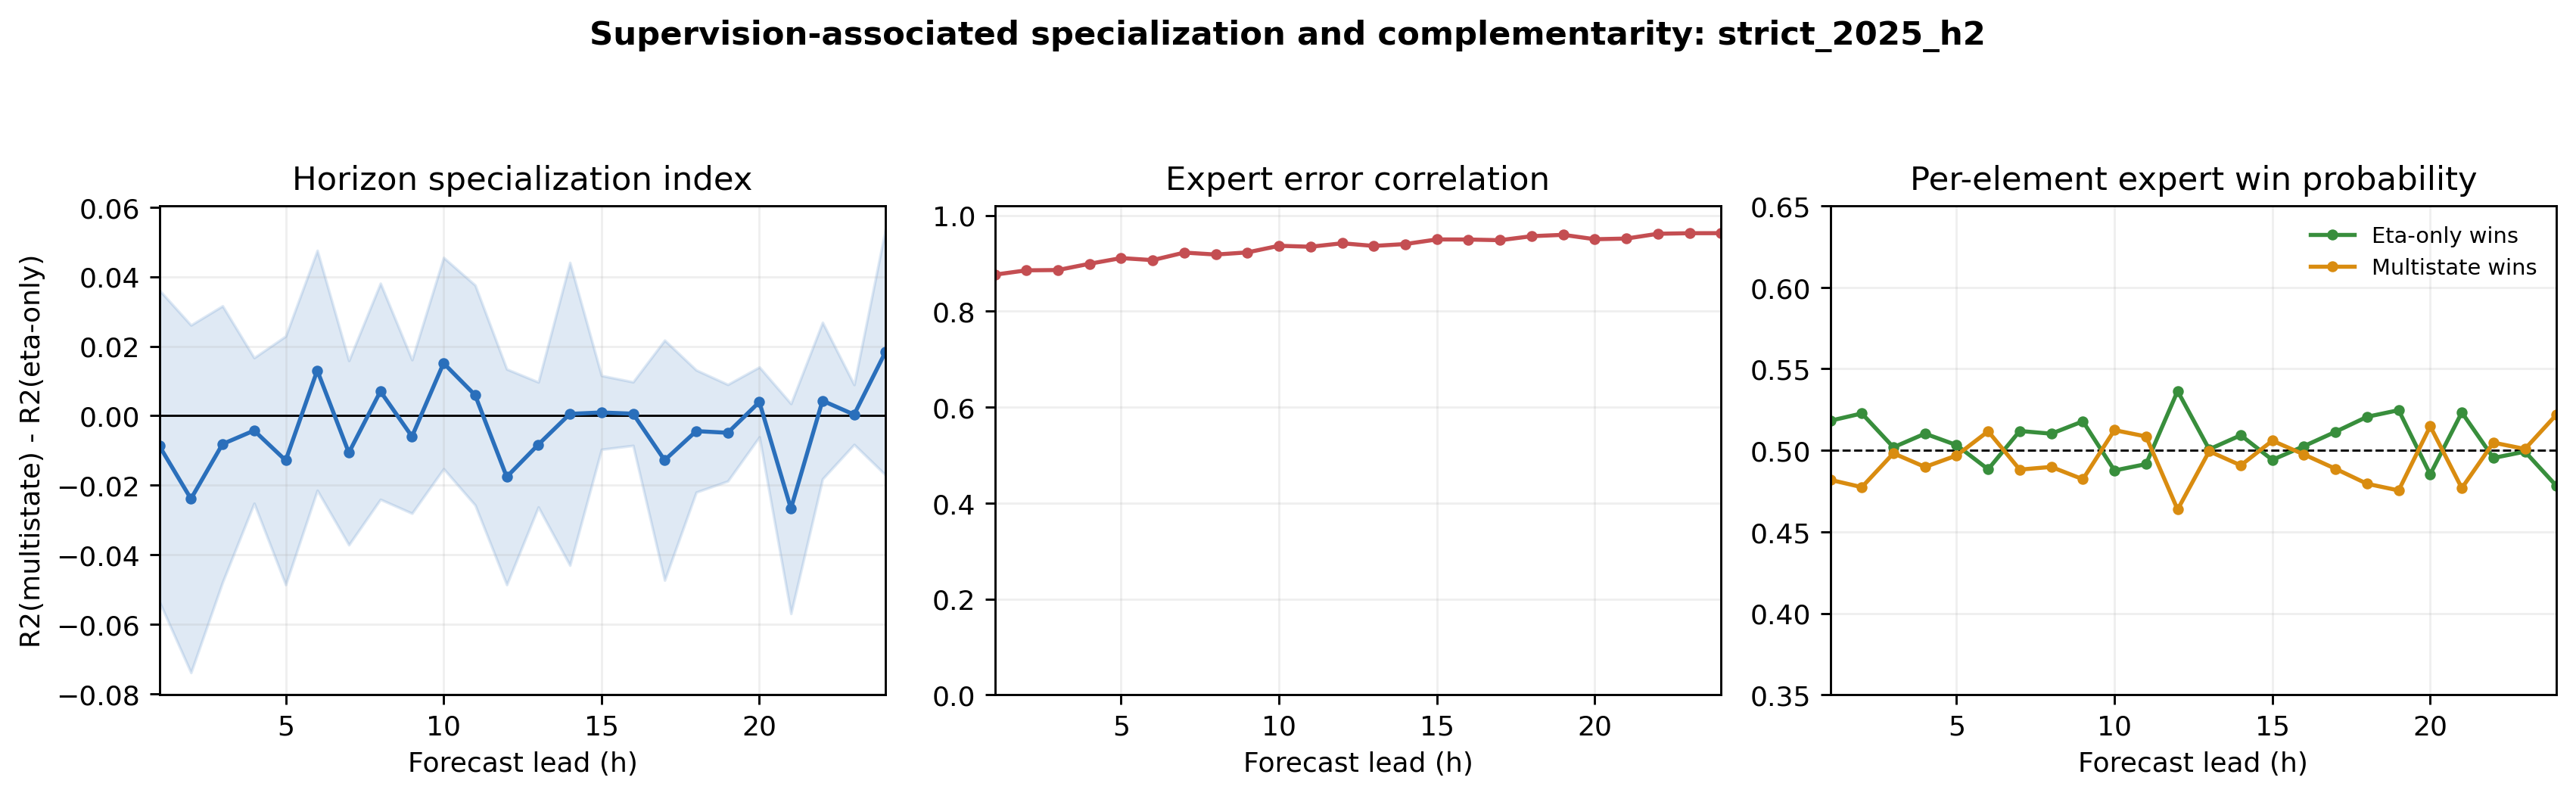
\includegraphics[width=0.98\textwidth]{fig3_specialization_complementarity.png}
\caption{Strict 2025 H2 supervision analysis. The horizon specialization index alternates in sign, errors are highly but imperfectly correlated, and neither expert wins every element. Shading denotes cross-seed variability.}
\label{fig:specialization}
\end{figure*}

Station-level structure is clearer (Fig.~\ref{fig:heatmap}). Multistate supervision is positive at lead 24 across all seven stations, whereas several earlier leads favor eta-only prediction. The location and sign of specialization vary across stations, which argues for a structured but region-dependent effect rather than a universal horizon rule.

\begin{figure*}[t]
\centering
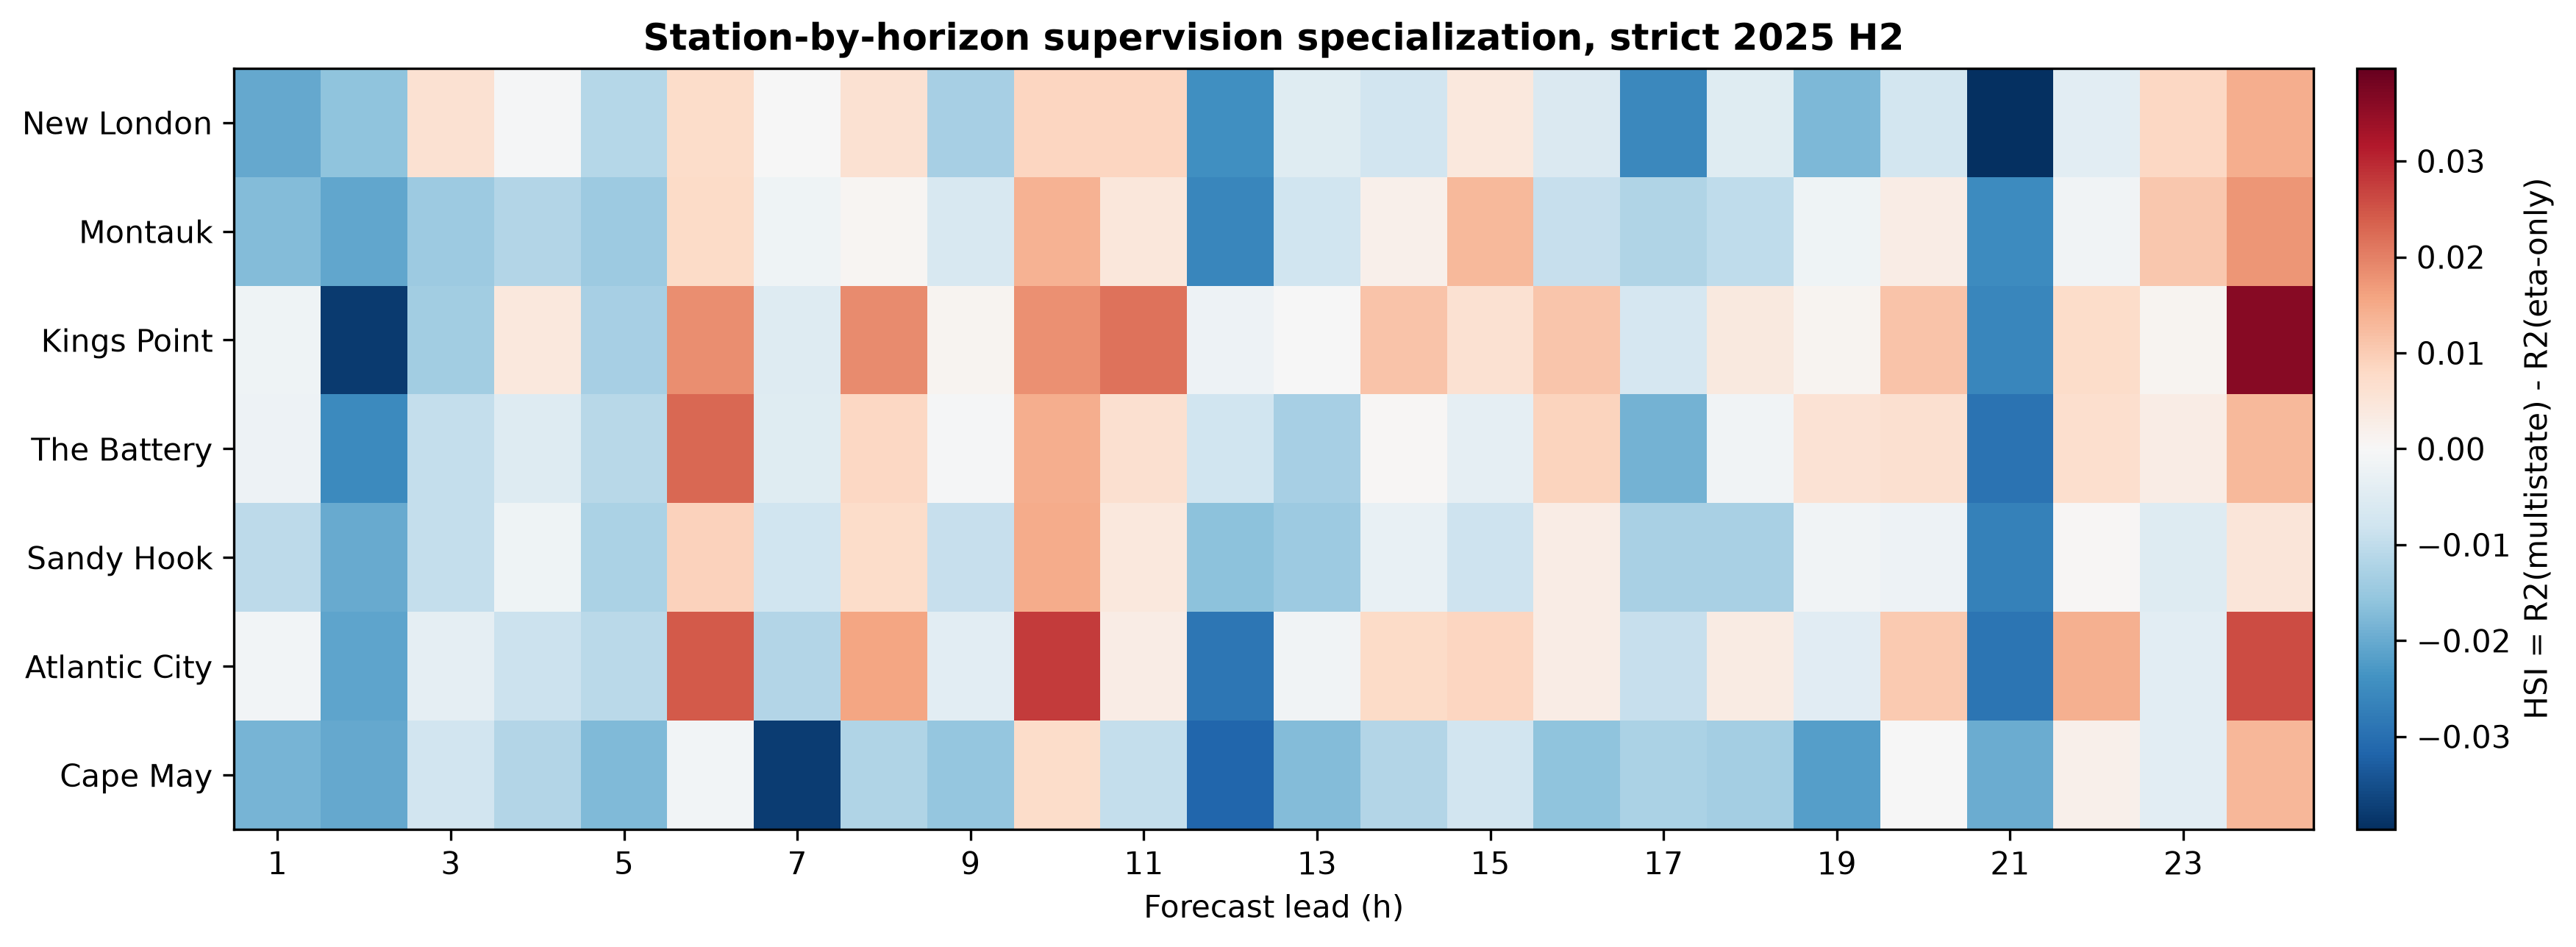
\includegraphics[width=0.94\textwidth]{fig4_station_horizon_specialization.png}
\caption{Five-seed mean station-by-horizon specialization in strict 2025 H2. Red favors the multistate expert and blue favors eta-only prediction.}
\label{fig:heatmap}
\end{figure*}

\subsection{A frozen low-complexity expert combination improves deep sequence skill}
HS-DT reaches sequence $R^2=0.6563$ in the 2025 H2 refit, improving over eta-only by 0.00915 and multistate by 0.01243; all five seeds improve in both comparisons, and the corresponding 168-h block intervals are [0.00141, 0.01955] and [0.00371, 0.02124]. In frozen 2026 H1, HS-DT improves over multistate by 0.01525 (5/5 seeds; block interval [0.00828, 0.02165]). July gives 0.01773 (5/5; interval [0.00907, 0.02839]). The lead-24 output remains exactly the multistate expert by design.

These results support transfer of the sequence-averaging effect, not a claim that HS-DT is best at every lead or upper-tail subset. July descriptive $q95$ values are strongly negative for all deep models, and HS-DT does not provide a stable extreme advantage.

\subsection{Prospectively locked spatial confirmation separates transferable and regional effects}
All ten Delaware stations pass the frozen coverage gate, so no station is removed after scoring. Table~\ref{tab:external} reports the 2025 H2 external test. VARX is the strongest sequence model at $R^2=0.7657$. HS-DT reaches $0.6803\pm0.0058$, improving over eta-only by $+0.01634$ in 5/5 seeds (168-h interval [0.00949, 0.02420]) and over multistate by $+0.00453$ in 4/5 seeds (interval [-0.00144, 0.01012]). The latter satisfies the locked positive-point-effect criterion but is not an uncertainty-separated gain. Lead 24 remains exactly the multistate output by design.

\begin{table*}[t]
\centering
\caption{Tier-D Delaware Bay--River spatial confirmation. Neural values are means $\pm$ standard deviations over five seeds; VARX is deterministic.}
\label{tab:external}
\small
\begin{tabular}{lccc}
\toprule
Model & Sequence $R^2$ & Lead-24 $R^2$ & Lead-24 RMSE (m) \\
\midrule
VARX--Ridge & 0.7657 & 0.5763 & 0.1405 \\
Eta-only FS-GWN & 0.6639 $\pm$ 0.0115 & 0.5217 $\pm$ 0.0207 & 0.1493 $\pm$ 0.0032 \\
Multistate FS-GWN & 0.6757 $\pm$ 0.0061 & 0.5743 $\pm$ 0.0105 & 0.1409 $\pm$ 0.0017 \\
HS-DT-GWN & 0.6803 $\pm$ 0.0058 & 0.5743 $\pm$ 0.0105 & 0.1409 $\pm$ 0.0017 \\
\bottomrule
\end{tabular}
\end{table*}

The original-region specialization pattern does not replicate. Eta-only wins only Leads 1 and 5, multistate wins the remaining 22 leads, and multistate wins sequence $R^2$ at all ten stations. Thus supervision-associated differences are real in the evaluated data but their topology is regional rather than a universal task partition. The third criterion does replicate at the curve level: on predictions averaged across the five seeds, HS-DT trails VARX by 0.11845 $R^2$ on average over Leads 1--8 but exceeds VARX by 0.01334 at Lead 24. This is not a 5/5 single-run terminal result: only two of five multistate/HS-DT runs exceed deterministic VARX at Lead 24. Overall, two of three locked criteria pass (Fig.~\ref{fig:external}), meeting the predeclared confirmation rule while retaining the failed specialization criterion.

\begin{figure*}[t]
\centering
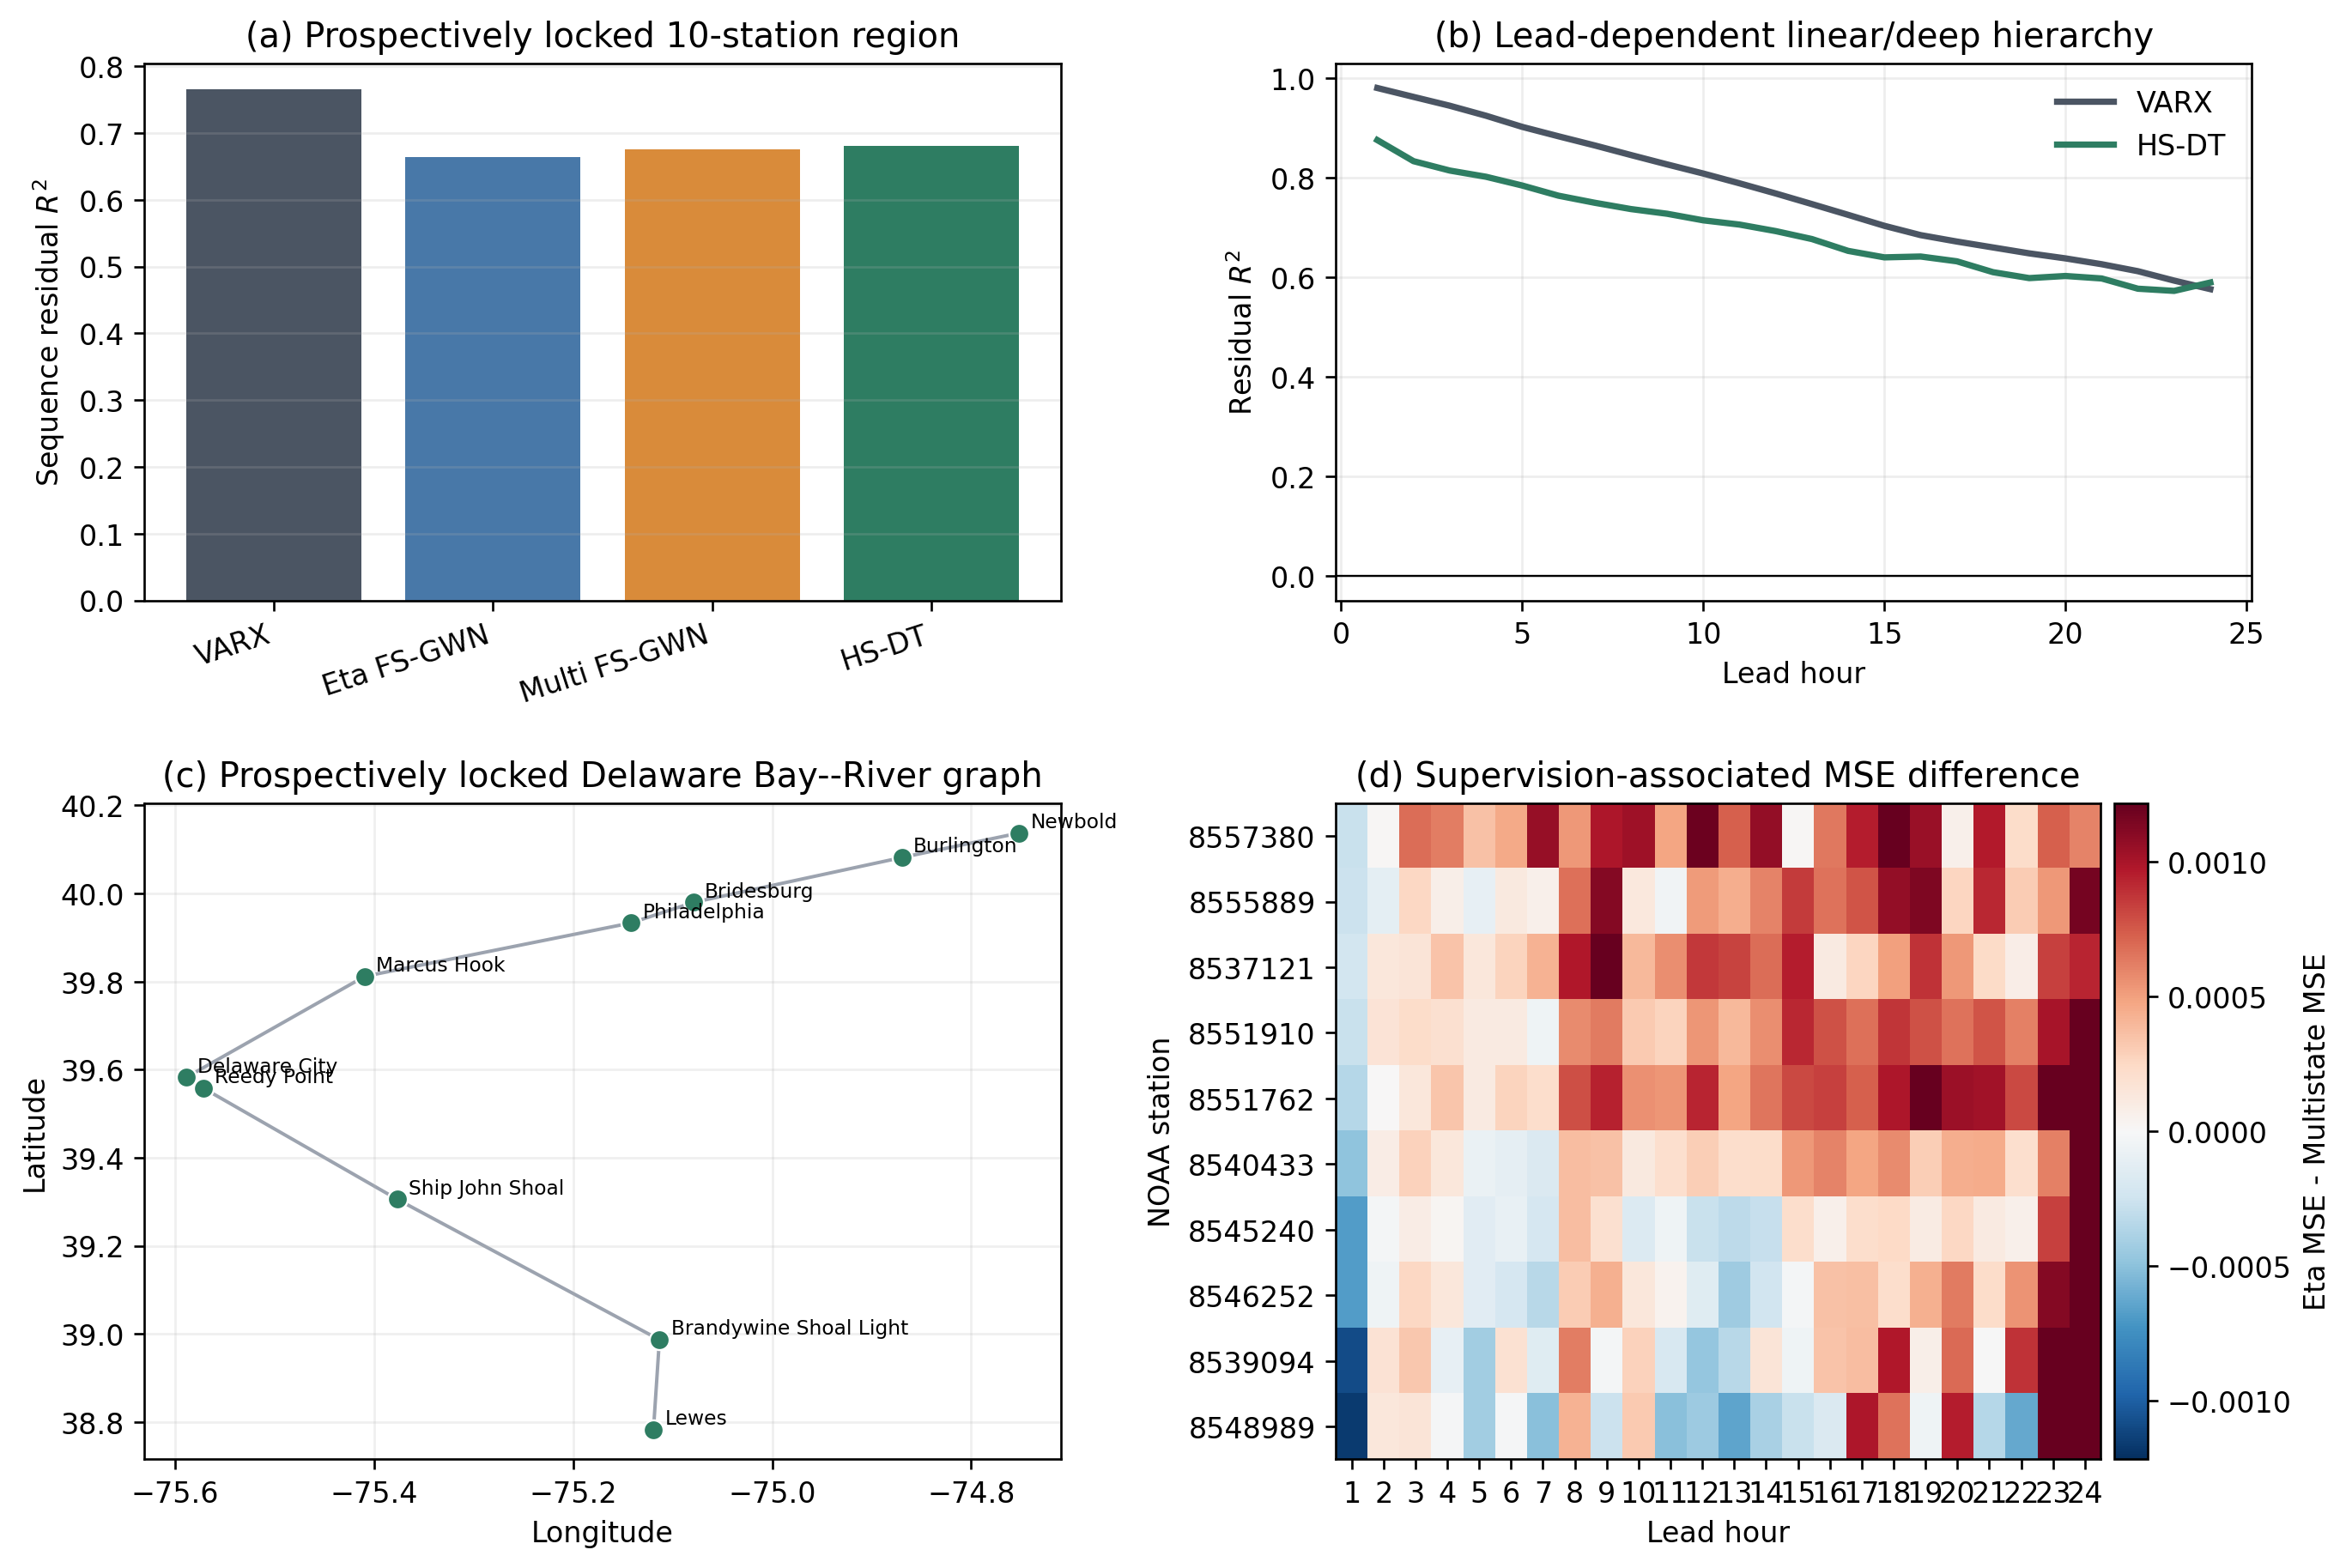
\includegraphics[width=0.98\textwidth]{fig7_external_region_confirmation.png}
\caption{Prospectively locked spatial confirmation. VARX remains the strongest external sequence model; the linear--deep ordering changes only at the far lead. Multistate supervision dominates most leads and every station, so the original-region station-wise specialization pattern does not replicate. Panel (d) shows eta MSE minus multistate MSE; positive values favor multistate.}
\label{fig:external}
\end{figure*}

\subsection{The observed linear--deep hierarchy changes across periods and horizons}
Table~\ref{tab:temporal} and Fig.~\ref{fig:hierarchy} expose the central robustness result. VARX dominates all 24 mean lead curves in 2025 H2 and has a 0.0582 sequence advantage over HS-DT. The diagnostic 2026 overlay reverses the ranking: HS-DT exceeds VARX by 0.1070 in H1 and 0.0441 in July. VARX remains strong at early leads, crosses the deep curves around leads 9--13, and becomes negative at lead 24 in both 2026 periods.

\begin{table*}[t]
\centering
\caption{Temporal evidence tiers. Neural entries are five-seed means. The 2026 HS-DT comparisons were frozen evaluations; the later-added VARX values are diagnostic-only because those targets had already been viewed.}
\label{tab:temporal}
\small
\begin{tabular}{llcccc}
\toprule
Period & Evidence status & Eta-only GWN & Multistate GWN & HS-DT-GWN & VARX-Ridge \\
\midrule
2025 H2 & chronological refit & 0.6472 & 0.6439 & 0.6563 & \textbf{0.7146} \\
2026 H1 & frozen deep; VARX diagnostic & 0.5185 & 0.5232 & \textbf{0.5385} & 0.4315 \\
2026 July & frozen deep; VARX diagnostic & 0.3915 & 0.3916 & \textbf{0.4093} & 0.3653 \\
\bottomrule
\end{tabular}
\end{table*}

\begin{figure*}[t]
\centering
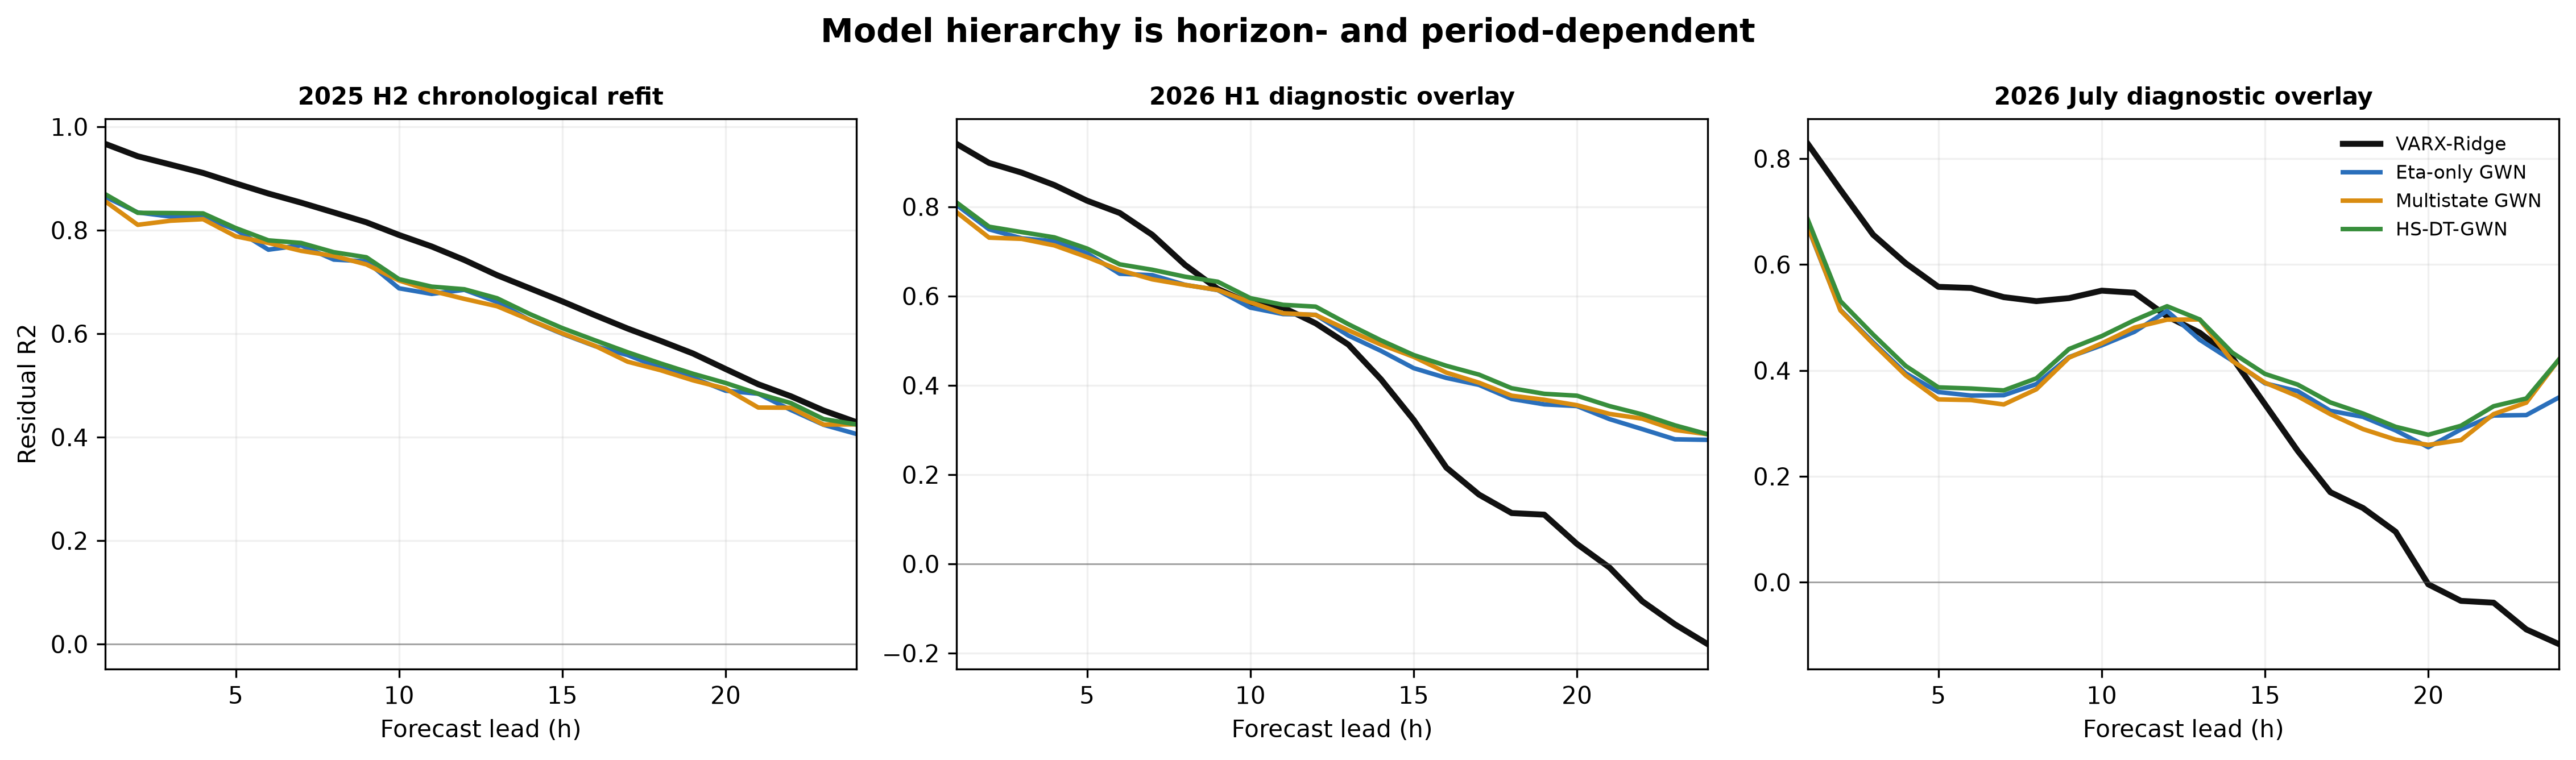
\includegraphics[width=0.99\textwidth]{fig5_temporal_hierarchy.png}
\caption{Lead-wise model hierarchy across periods. VARX dominates strict 2025 H2 and the early leads of 2026, but its far-lead skill collapses in 2026. The 2026 VARX overlay is diagnostic-only.}
\label{fig:hierarchy}
\end{figure*}

The observed result rejects two simple descriptions of these evaluated periods. Linear modeling does not uniformly eliminate the need for graph-temporal models, and deep modeling does not uniformly dominate a strong low-variance baseline. The hierarchy depends jointly on temporal regime and forecast lead, but the 2026 VARX overlay requires prospective confirmation.

\subsection{Physical priors have architecture- and task-conditional marginal utility}
Table~\ref{tab:physics} reports matched continuous-metric effects. Direct physical loss reduces strict GNN--BiGRU sequence and lead-24 $R^2$. Joint ODE injection gives a small sequence increment over the same-capacity GWN control ($+0.00444$; 4/5 seeds) but decreases Lead-24. Dual ODE injection behaves similarly for HS-DT ($+0.00221$ sequence; 4/5 seeds; negative Lead-24). Adding direct physical loss after ODE injection is effectively zero. Effect magnitudes and mixed directions, rather than five-seed significance, support the narrow attribution claim.

\begin{table*}[t]
\centering
\caption{Matched physical-prior effects. Positive changes favor the physical variant.}
\label{tab:physics}
\small
\begin{tabular}{llrrrl}
\toprule
Protocol & Comparison & $\Delta$ sequence $R^2$ & $\Delta$ lead-24 $R^2$ & $\Delta q95$ $R^2$ & Interpretation \\
\midrule
Strict H2 & GNN direct loss -- no loss & -0.00402 & -0.00722 & -0.01538 & nonpositive \\
Strict H2 & GWN joint ODE -- capacity control & +0.00444 & -0.00847 & +0.00558 & mixed, nonsignificant \\
Strict H2 & HS-DT dual ODE -- capacity control & +0.00221 & -0.00847 & +0.00192 & mixed, nonsignificant \\
Strict H2 & direct loss on ODE HS-DT & +0.000002 & +0.000027 & +0.000011 & effectively zero \\
Retrospective & GWN direct loss -- no loss & -0.000119 & -0.000232 & -0.000536 & matched nonpositive \\
\bottomrule
\end{tabular}
\end{table*}

In the retrospective high-forcing $q95$ subset, the ODE residual correction reduces MSE by 1.06\% relative to the unadapted HS-DT prediction (5/5 seeds), but only 0.30\% relative to a zero-signal adapter (4/5) and 0.07\% relative to a persistence adapter (4/5). The larger headline contrast is therefore capacity-confounded. Figure~\ref{fig:physics} keeps strict matched attribution and retrospective regime effects visually separate; the full lead-wise audit is supplied with the result tables.

\begin{figure*}[t]
\centering
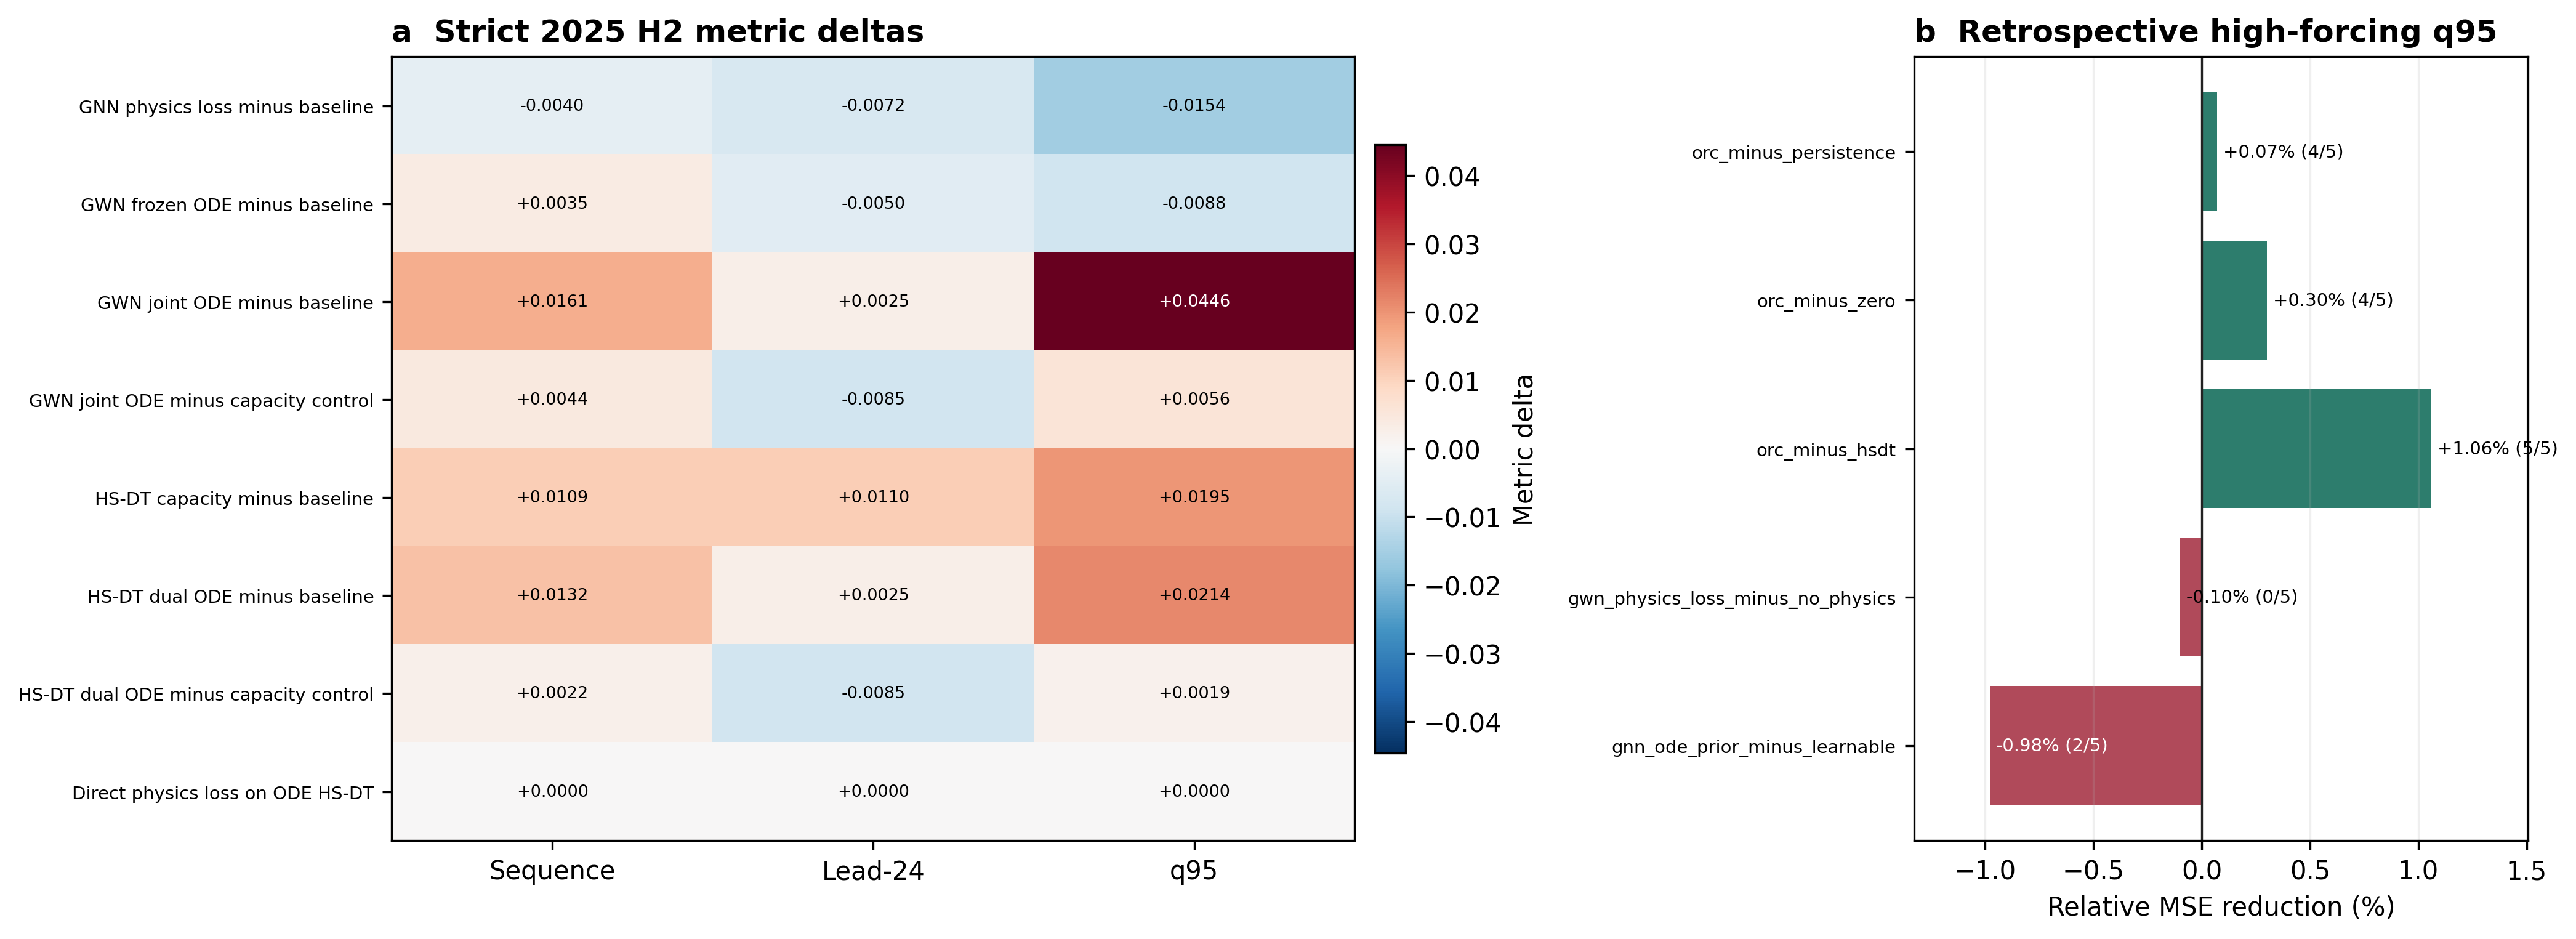
\includegraphics[width=0.96\textwidth]{fig6_physics_utility_mainline.png}
\caption{Architecture-conditional physics utility. Panel (a) reports strict continuous-metric deltas; panel (b) reports retrospective high-forcing diagnostics. Capacity-only and capacity-confounded rows are retained to prevent attribution of joint gains to physics alone. Event classification is excluded from the mainline.}
\label{fig:physics}
\end{figure*}

\subsection{Increasing complexity does not guarantee temporal transfer}
Several high-capacity or post-hoc candidates fail predeclared transfer checks (Table~\ref{tab:boundary}). These negative controls define a useful complexity boundary: additional freedom is not evidence of additional transferable forecast skill.

\begin{table*}[t]
\centering
\caption{Complexity-boundary evidence.}
\label{tab:boundary}
\footnotesize
\begin{tabular}{p{0.25\textwidth}p{0.64\textwidth}}
\toprule
Candidate & Diagnostic result \\
\midrule
Reliability/uncertainty router & best expert-win AUROC about 0.552 \\
Safety-gated dual head & continuous skill decreases in July \\
Terminal physics adapter & does not beat the horizon-only anchor \\
Residual booster & zero correction selected at epoch 0 after checkpoint repair \\
CF-MOR P0 proxy & confirmation residual $R^2=-0.0935$; epoch 0 \\
Validation-safe lead mask & selected mask reduces test sequence skill \\
\bottomrule
\end{tabular}
\end{table*}

\clearpage
\section{Discussion}
\subsection{What is transferable in the current evidence}
Three findings survive the expanded baseline set. First, Graph WaveNet supplies the strongest deep temporal backbone. Second, eta-only and multistate supervision produce related but nonidentical errors, and a fixed low-complexity combination repeatedly improves sequence point estimates. The external region strengthens the complementarity claim but rejects a universal specialization map: it favors multistate at 22 of 24 leads and all ten stations. Third, model-family ranking is horizon-dependent. VARX remains excellent overall and at early leads, while the five-seed mean deep curve retains slightly more Lead-24 skill externally.

The physical result is intentionally narrower. Simplified priors can alter particular horizons or high-forcing subsets, but matched controls remove most apparent gains. Multistate supervision may already expose the network to current and wave information that a simplified residual would otherwise encourage indirectly. A stronger backbone can likewise absorb relationships represented by a low-order prior.

\subsection{Implications for model selection}
A single average score conceals horizon-dependent failure. VARX would be selected from 2025 H2 sequence skill, yet its 2026 lead-24 $R^2$ is negative. Conversely, HS-DT is not the 2025 H2 winner but is more stable at later far leads. Operational selection should therefore be conditioned on lead, forcing availability, and temporal regime, with a validation-locked fallback rather than a test-selected router.

The fixed HS-DT rule is intentionally simple. Its contribution is evidence that complementary supervision can be used with low selection freedom. It is not proposed as a universal routing optimum. A future probabilistic mixture should be trained and frozen on genuinely unseen development data, then evaluated once on a later target period.

\subsection{Limitations and external confirmation}
The primary graph contains only seven nodes in one coastal region. Tier D reduces this limitation with ten non-overlapping stations, but both regions remain in the U.S. Mid-Atlantic and use the same 2025 H2 calendar test period; it tests spatial replication and graph-size sensitivity, not global generality or later-period temporal transfer. Daily current and three-hourly wave products are aligned to an hourly grid, and the retrospective benchmark includes forcing availability that is more favorable than issue-time operations. Local NOAA meteorology has substantial missingness. The descriptive $q95$ subset is not a storm-surge event definition, and July upper-tail $R^2$ is unstable because the subset is small and low variance.

The strict original-region 2025 H2 period was viewed during development. The GWN and HS-DT 2026 evaluations were frozen, but the original-region VARX overlay was designed after those outcomes and remains diagnostic. Tier D provides prospectively locked spatial confirmation, not a later-period temporal holdout. Its protocol was hash-locked locally rather than registered with an independent repository, and the Lead 1--8 implementation of ``early'' was documented before external neural scoring but after the initial protocol hash. A future decisive experiment should preregister exact lead groups publicly and score all model families once on a later untouched period or a more distant hydrographic regime.

\section{Reproducibility}
The Overleaf package includes the exact summary tables used for specialization, temporal hierarchy, HS-DT paired comparisons, matched physics attribution, and external confirmation, together with the machine-readable decision, frozen protocol, and technical-repair ledger. Preprocessing fits scalers and learned graphs only on the training period in causal experiments. Neural comparisons use paired seeds and identical windows. A code audit before external neural scoring found and removed a second bounded carry on 17 derived local-meteorology values; all formal models were rerun from regenerated hashes, and pre-repair outputs were quarantined. Smoke, partial, obsolete $\lambda=0.0003$, and superseded PDF results are excluded. The locked physical-loss weight is $\lambda=0.0002$.

\section{Conclusions}
This study reframes coastal residual forecasting from a search for one complex champion into a controlled analysis of transferable mechanisms and their boundaries. Graph WaveNet is the strongest deep backbone, and fixed HS-DT fusion repeatedly improves deep sequence point estimates. Prospectively locked ten-station spatial confirmation passes two of three declared criteria: low-complexity expert complementarity and lead-dependent VARX--deep ordering replicate, whereas the original station-wise supervision pattern does not. VARX remains the strongest external sequence model, so the result is horizon-dependent complementarity rather than deep-model dominance. Matched controls show that the tested physical priors have small, mixed, architecture- and task-conditional marginal utility. The next requirement is a publicly preregistered later-period or more distant-region test, especially for the modest HS-DT-over-multistate effect whose external block interval crosses zero.

\section*{Data availability}
Raw water-level and local observations are available from NOAA CO-OPS and NDBC; atmospheric reanalysis from the Copernicus Climate Data Store; ocean and wave products from Copernicus Marine; and bathymetry from GEBCO. Distribution of derived arrays remains subject to source-product terms.

\section*{Declaration of competing interest}
The authors declare no known competing financial interests or personal relationships that could have appeared to influence the work reported in this paper.

\section*{Acknowledgements}
Removed for anonymous review.

\bibliographystyle{elsarticle-harv}
\bibliography{references}
\end{document}
